\documentclass{bmcart}

%%%%%%%%%%%%%%%%%%%%%%%%%%%%%%%%%%%%%%%%%%%%%%
%%                                          %%
%% CARGA DE PAQUETES DE LATEX               %%
%%                                          %%
%%%%%%%%%%%%%%%%%%%%%%%%%%%%%%%%%%%%%%%%%%%%%%

%%% Load packages
\usepackage{amsthm,amsmath}
\usepackage{graphicx}
%\RequirePackage[numbers]{natbib}
%\RequirePackage{hyperref}
\usepackage[utf8]{inputenc} %unicode support
%\usepackage[applemac]{inputenc} %applemac support if unicode package fails
%\usepackage[latin1]{inputenc} %UNIX support if unicode package fails
\usepackage{hyperref}


%%%%%%%%%%%%%%%%%%%%%%%%%%%%%%%%%%%%%%%%%%%%%%
%%                                          %%
%% COMIENZO DEL DOCUMENTO                   %%
%%                                          %%
%%%%%%%%%%%%%%%%%%%%%%%%%%%%%%%%%%%%%%%%%%%%%%

\begin{document}

	\begin{frontmatter}
	
		\begin{fmbox}
			\dochead{Research}
			
			%%%%%%%%%%%%%%%%%%%%%%%%%%%%%%%%%%%%%%%%%%%%%%
			%% INTRODUCIR TITULO PROYECTO               %%
			%%%%%%%%%%%%%%%%%%%%%%%%%%%%%%%%%%%%%%%%%%%%%%
			
			\title{Respuesta a la infección por SARS-CoV2}
			
			%%%%%%%%%%%%%%%%%%%%%%%%%%%%%%%%%%%%%%%%%%%%%%
			%% AUTORES. METER UNA ENTRADA AUTHOR        %%
			%% POR PERSONA                              %%
			%%%%%%%%%%%%%%%%%%%%%%%%%%%%%%%%%%%%%%%%%%%%%%
			
			\author[
			  addressref={aff1},                   % ESTA LINEA SE COPIA IGUAL PARA CADA AUTOR
			  corref={aff1},                       % ESTA LINEA SOLO DEBE TENERLA EL COORDINADOR DEL GRUPO
			  email={carmenarrabali@uma.es}  		% VUESTRO CORREO ACTIVO
			]{\inits{C.L.A.C.}\fnm{Carmen Lucía} \snm{Arrabalí Cañete}} % inits: INICIALES DE AUTOR, fnm: NOMBRE DE AUTOR, snm: APELLIDOS DE AUTOR
			
			\author[
			  addressref={aff1},
			  email={olegbrz@uma.es}
			]{\inits{O.B.}\fnm{Oleg} \snm{Brezitskyy}}
			
			\author[
			addressref={aff1},
			email={correo de juan}
			]{\inits{J.A.H.C.}\fnm{Juan Antonio} \snm{Herrera Conde}}
			
			\author[
			addressref={aff1},
			email={correo de sergio}
			]{\inits{S.M.V.}\fnm{Sergio} \snm{Martin Vera}}
			
			
			%%%%%%%%%%%%%%%%%%%%%%%%%%%%%%%%%%%%%%%%%%%%%%
			%% AFILIACION. NO TOCAR                     %%
			%%%%%%%%%%%%%%%%%%%%%%%%%%%%%%%%%%%%%%%%%%%%%%
			
			\address[id=aff1]{%                           % unique id
			  \orgdiv{ETSI Informática},             % department, if any
			  \orgname{Universidad de Málaga},          % university, etc
			  \city{Málaga},                              % city
			  \cny{España}                                    % country
			}
		
		\end{fmbox}% comment this for two column layout
		
		\begin{abstractbox}
		
			\begin{abstract} % abstract
			
			%%%%%%%%%%%%%%%%%%%%%%%%%%%%%%%%%%%%%%%%%%%%%%%
			%% RESUMEN BREVE DE NO MAS DE 100 PALABRAS   %%
			%%%%%%%%%%%%%%%%%%%%%%%%%%%%%%%%%%%%%%%%%%%%%%%	
			
			\end{abstract}
			
			%%%%%%%%%%%%%%%%%%%%%%%%%%%%%%%%%%%%%%%%%%%%%%
			%% PALABRAS CLAVE DEL PROYECTO              %%
			%%%%%%%%%%%%%%%%%%%%%%%%%%%%%%%%%%%%%%%%%%%%%%
			
			\begin{keyword}
			\kwd{SARS-CoV-2}
			\kwd{COVID-19}
			\kwd{Coronavirus}
			\end{keyword}
		
		
		\end{abstractbox}
	
	\end{frontmatter}
	
	%%%%%%%%%%%%%%%%%%%%%%%%%%%%%%%%%%%%%%%%%%%%%%%%%%%%%%%%%%%%%%%%%%%%%%%%%%%%%%%%%%%%%%%%
	%% EJEMPLO DE LATEX %%                                                                %%
	%% BORRAR ANTES DE ENTREGAR!!!!!!!!!!!!!!!!!!!!!!!!!!!!!!!!!!!!!!!!!!!!!              %%
	%%%%%%%%%%%%%%%%%%%%%%%%%%%%%%%%%%%%%%%%%%%%%%%%%%%%%%%%%%%%%%%%%%%%%%%%%%%%%%%%%%%%%%%%
	
	\section*{Content}
		Text and results for this section, as per the individual journal's instructions for authors. Here, we reference the figure \ref{fig:cost_genome} and figure \ref{fig:cost_megabase} but also the table \ref{tab:ejemplo}.
	
	\section*{Section title}
		Text for this section\ldots

		In this section we examine the growth rate of the mean of $Z_0$, $Z_1$ and $Z_2$. In
		addition, we examine a common modeling assumption and note the
		importance of considering the tails of the extinction time $T_x$ in
		studies of escape dynamics.
		We will first consider the expected resistant population at $vT_x$ for
		some $v>0$, (and temporarily assume $\alpha=0$)
		%
		\[
		E \bigl[Z_1(vT_x) \bigr]=
		\int_0^{v\wedge
			1}Z_0(uT_x)
		\exp (\lambda_1)\,du .
		\]
		%
		If we assume that sensitive cells follow a deterministic decay
		$Z_0(t)=xe^{\lambda_0 t}$ and approximate their extinction time as
		$T_x\approx-\frac{1}{\lambda_0}\log x$, then we can heuristically
		estimate the expected value as
		%
		\begin{equation}\label{eqexpmuts}
			\begin{aligned}[b]
				&      E\bigl[Z_1(vT_x)\bigr]\\
				&\quad      = \frac{\mu}{r}\log x
				\int_0^{v\wedge1}x^{1-u}x^{({\lambda_1}/{r})(v-u)}\,du .
			\end{aligned}
		\end{equation}
		%
		%%%%%%%%%%%%%%%%%%%%%%%%%%%%%%%%%%%%%%%%%%%%%%%%%%%%%%%%%%%%%%%%%%%%%%
		%% USAR \cite{...} PARA INCLUIR REFERENCIAS BIBLIOGRAFICAS          %%
		%%  \cite{koon}  Para una sola                                      %%
		%%  \cite{oreg,khar,zvai,xjon,schn,pond} Para una lista             %%
		%%%%%%%%%%%%%%%%%%%%%%%%%%%%%%%%%%%%%%%%%%%%%%%%%%%%%%%%%%%%%%%%%%%%%%
		Thus we observe that this expected value is finite for all $v>0$ (also see \cite{koon,xjon,marg,schn,koha,issnic}).
		
		
		%%%%%%%%%%%%%%%%%%%%%%%%%%%%%%%%%%%%%%%%%%%%%%%%%%%%%%%%%%%%%%%%%%%%%%%%%%%%%%%%%%%%%%%%%%%
		%% FIGURAS                                                                               %%
		%% includegraphics: inserta la imagen                                                    %%
		%% caption: descripcion de la figura                                                     %%
		%% label: etiqueta para hacer referencia a la figura en el texto con la instrucción ref  %%
		%%%%%%%%%%%%%%%%%%%%%%%%%%%%%%%%%%%%%%%%%%%%%%%%%%%%%%%%%%%%%%%%%%%%%%%%%%%%%%%%%%%%%%%%%%%	
		
		\begin{figure}[h!]
			\includegraphics[width=0.9\textwidth]{figures/Sequencing_Cost_per_Genome_May2020.jpg}
			\caption{Sample figure title}
			\label{fig:cost_genome}
		\end{figure}
		
		\begin{figure}[h!]
			\includegraphics[width=0.9\textwidth]{figures/Sequencing_Cost_per_Megabase_May2020.jpg}
			\caption{Sample figure title}
			\label{fig:cost_megabase}
		\end{figure}
		
		%%%%%%%%%%%%%%%%%%%%%%%%%%%%%%%%%%%%%%%%%%%%%%%%%%%%%%%%%%%%%%%%%%%%%%%%%%%%%%%%%%%%%%%%%%
		%% TABLAS                                                                               %%
		%% caption: Descripción tabla                                                           %%
		%% \begin{tabular}{letras}: Indica numero de columnas.                                  %%
		%%    Una letra por columna, la letra indica la alineación de la columna:               %%
		%%    c center, l left, r right                                                         %%
		%% hline: Representa una linea como entre filas                                         %%
		%% \\: fin de fila                                                                      %%
		%% &: delimitador de celda                                                              %%
		%% label: etiqueta para hacer referencia a la tabla en el texto con la instrucción ref  %%
		%%%%%%%%%%%%%%%%%%%%%%%%%%%%%%%%%%%%%%%%%%%%%%%%%%%%%%%%%%%%%%%%%%%%%%%%%%%%%%%%%%%%%%%%%%
		
		\begin{table}[h!]
			\caption{Sample table title. This is where the description of the table should go}
			\begin{tabular}{cccc}
				\hline
				& B1  &B2   & B3\\ 
				\hline
				A1 & 0.1 & 0.2 & 0.3\\
				A2 & ... & ..  & .\\
				A3 & ..  & .   & .\\ 
				\hline
				\label{tab:ejemplo}
			\end{tabular}
		\end{table}
				
		\subsection*{Sub-heading for section}
			Text for this sub-heading\ldots
	
			\subsubsection*{Sub-sub heading for section}
				Text for this sub-sub-heading\ldots
					
					\paragraph*{Sub-sub-sub heading for section}
						Text for this sub-sub-sub-heading\ldots
	
	%%%%%%%%%%%%%%%%%%%%%%%%%%%%%%%%%
	%% FIN DE EJEMPLO !!!!!!!!!!!! %%
	%%%%%%%%%%%%%%%%%%%%%%%%%%%%%%%%%
	
	%%%%%%%%%%%%%%%%%%%%%%%%%%%%%%%%%
	%% COMIENZO DEL DOCUMENTO REAL %%
	%%%%%%%%%%%%%%%%%%%%%%%%%%%%%%%%%
	
	\section{Introducción}
Los coronavirus son un grupo diverso de virus de ARN monocatenario de sentido positivo con una amplia gama de huéspedes vertebrados. Cuatro géneros comunes de coronavirus (alfa, beta, gamma y delta) circulan entre los vertebrados y causan enfermedades leves del tracto respiratorio superior en humanos y gastroenteritis en animales. Sin embargo, en las últimas dos décadas han surgido tres betacoronavirus humanos altamente patógenos a partir de eventos zoonóticos. En 2002-2003, el coronavirus 1 relacionado con el síndrome respiratorio agudo severo (SARS-CoV-1) infectó a $\approx$8000 personas en todo el mundo con una tasa de letalidad de $\approx$10\%, seguido por el coronavirus relacionado con el síndrome respiratorio de Oriente Medio (MERS-CoV), que ha infectado a $\approx$2500 personas con una tasa de letalidad de $\approx$36\% desde 2012. En la actualidad, el mundo sufre una pandemia de SARS-CoV-2, causante de la enfermedad por coronavirus 2019 (COVID-19) y tiene una tasa de mortalidad global que aún está por determinar.

La infección por SARS-CoV-2 se caracteriza por una variedad de síntomas que incluyen fiebre, tos y malestar general en la mayoría de los casos, pero en los casos más graves, pueden llegar a desarrollar un síndrome de dificultad respiratoria aguda y lesión pulmonar aguda, lo que provoca morbilidad y mortalidad causadas por daños en la luz alveolar que conducen a inflamación y neumonía.

Entendiendo qué respuesta puede tener el cuerpo cuando se infecta por SARS-CoV-2, ahora se estudiará esta respuesta, pero desarrollada en las células del epitelio del pulmón mediante el análisis de perfiles de expresión génica publicados en el dataset GEO GSE147507~\cite{BlancoMelo2020}.
	\section{Materiales y métodos}
\subsection{Carga de datos}
Para poder hacer uso de los datos que se anexan al artículo científico en el que está basado el proyecto, se han de descargar desde la página web del NCBI, con un archivo llamado \textit{setup.sh}. Por otro lado, hay un archivo llamado \textit{launch.sh} que se encarga de ejecutar todos los archivos de R. Se obtienen un total de 21797 genes con 79 muestras cada uno con los que se empieza el análisis.

\subsection{Análisis inicial}
Se crea el archivo llamado \textit{Análisis\_EG\_dataInput.R}, el cual carga los datos y se crea la limpieza y preprocesamiento de los datos. En primer lugar se crea una configuración del entorno de R y se procesan los datos. Se hace uso de la librería de \textit{WCGNA} obtenida desde \textit{Bioconductor}. 

Por otro lado se hace un reajuste de datos, se transforman para que sean las filas las correspondientes a los genes y, las columnas, a las muestras de los mismos.

Como se desconoce si hay alguna falta de datos, se comprueba si hay algún dato que falta o que es nulo. En el caso de que si haya datos no válidos, se eliminan los genes y las muestras de estos.

Luego, se agrupan para poder ver si hay o no valores atípicos y luego se eliminan aquellos que si que lo sean con un corte de altura. 

Todos los datos mencionados anteriormente se almacenan para poder hacer así el análisis de red.

\begin{figure}[h]
	\fbox{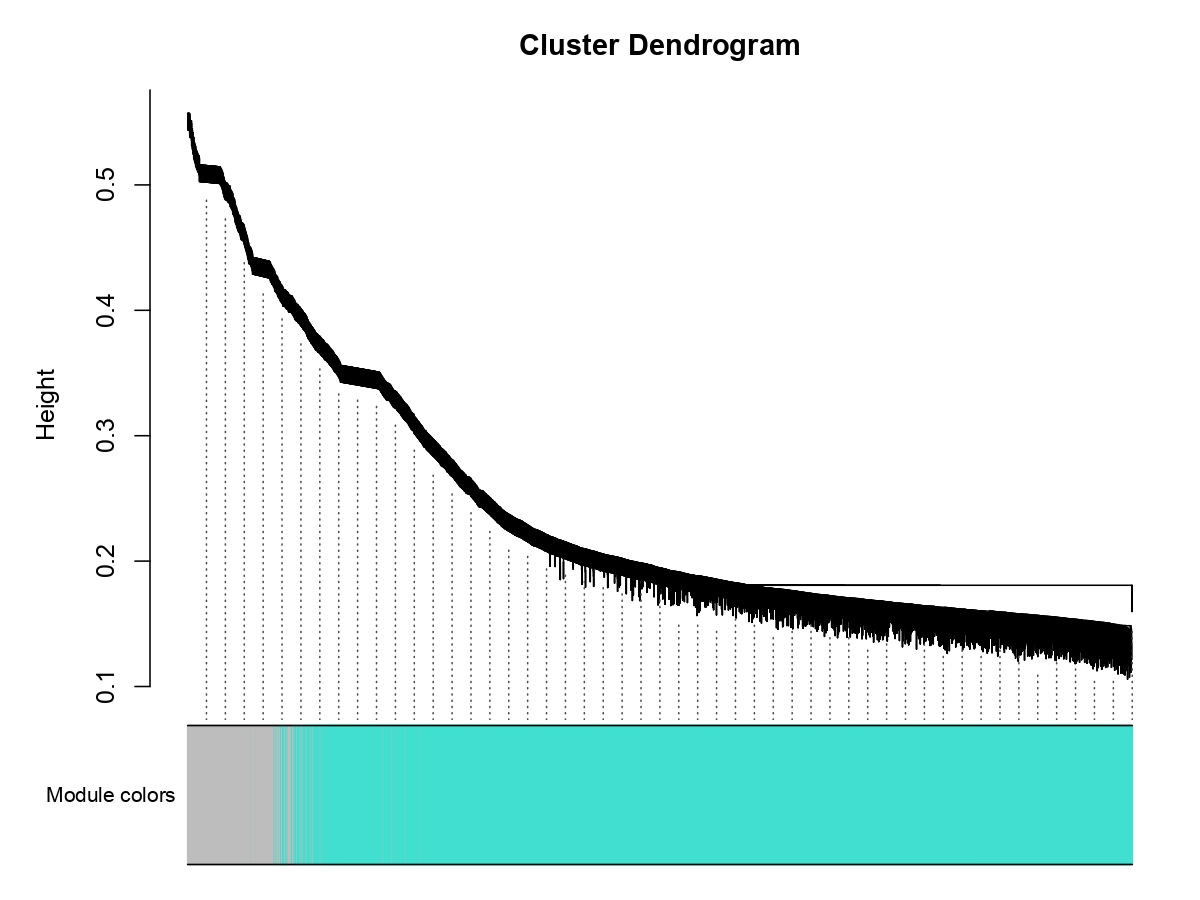
\includegraphics[width=0.9\textwidth]{figures/clusterDendrogram.jpg}}
	\caption{Cluster Dendrogram}
	\label{fig:clusterDendrogram}
\end{figure}


	
\section{Resultados}

Una vez instalados todos los paquetes y librerías necesarias, debemos empezar con la limpiza de datos y su preprocesamiento, por lo que cargamos el dataset de perfiles de expresión génica. Transformamos los datos para poder trabajar con filas y columnas, descubriendo así si hay genes con valores perdidos. Si la última comprobación devuelve \textit{TRUE}, no necesitaremos ejecutar el siguiente código. De lo contrario, se eliminan los genes, mostrándose prescindibles. Agrupamos las muestras para ver si hay valores atípicos y una vez detectados, los eliminamos eligiendo un corte de altura. 

\begin{figure}[h]
	\fbox{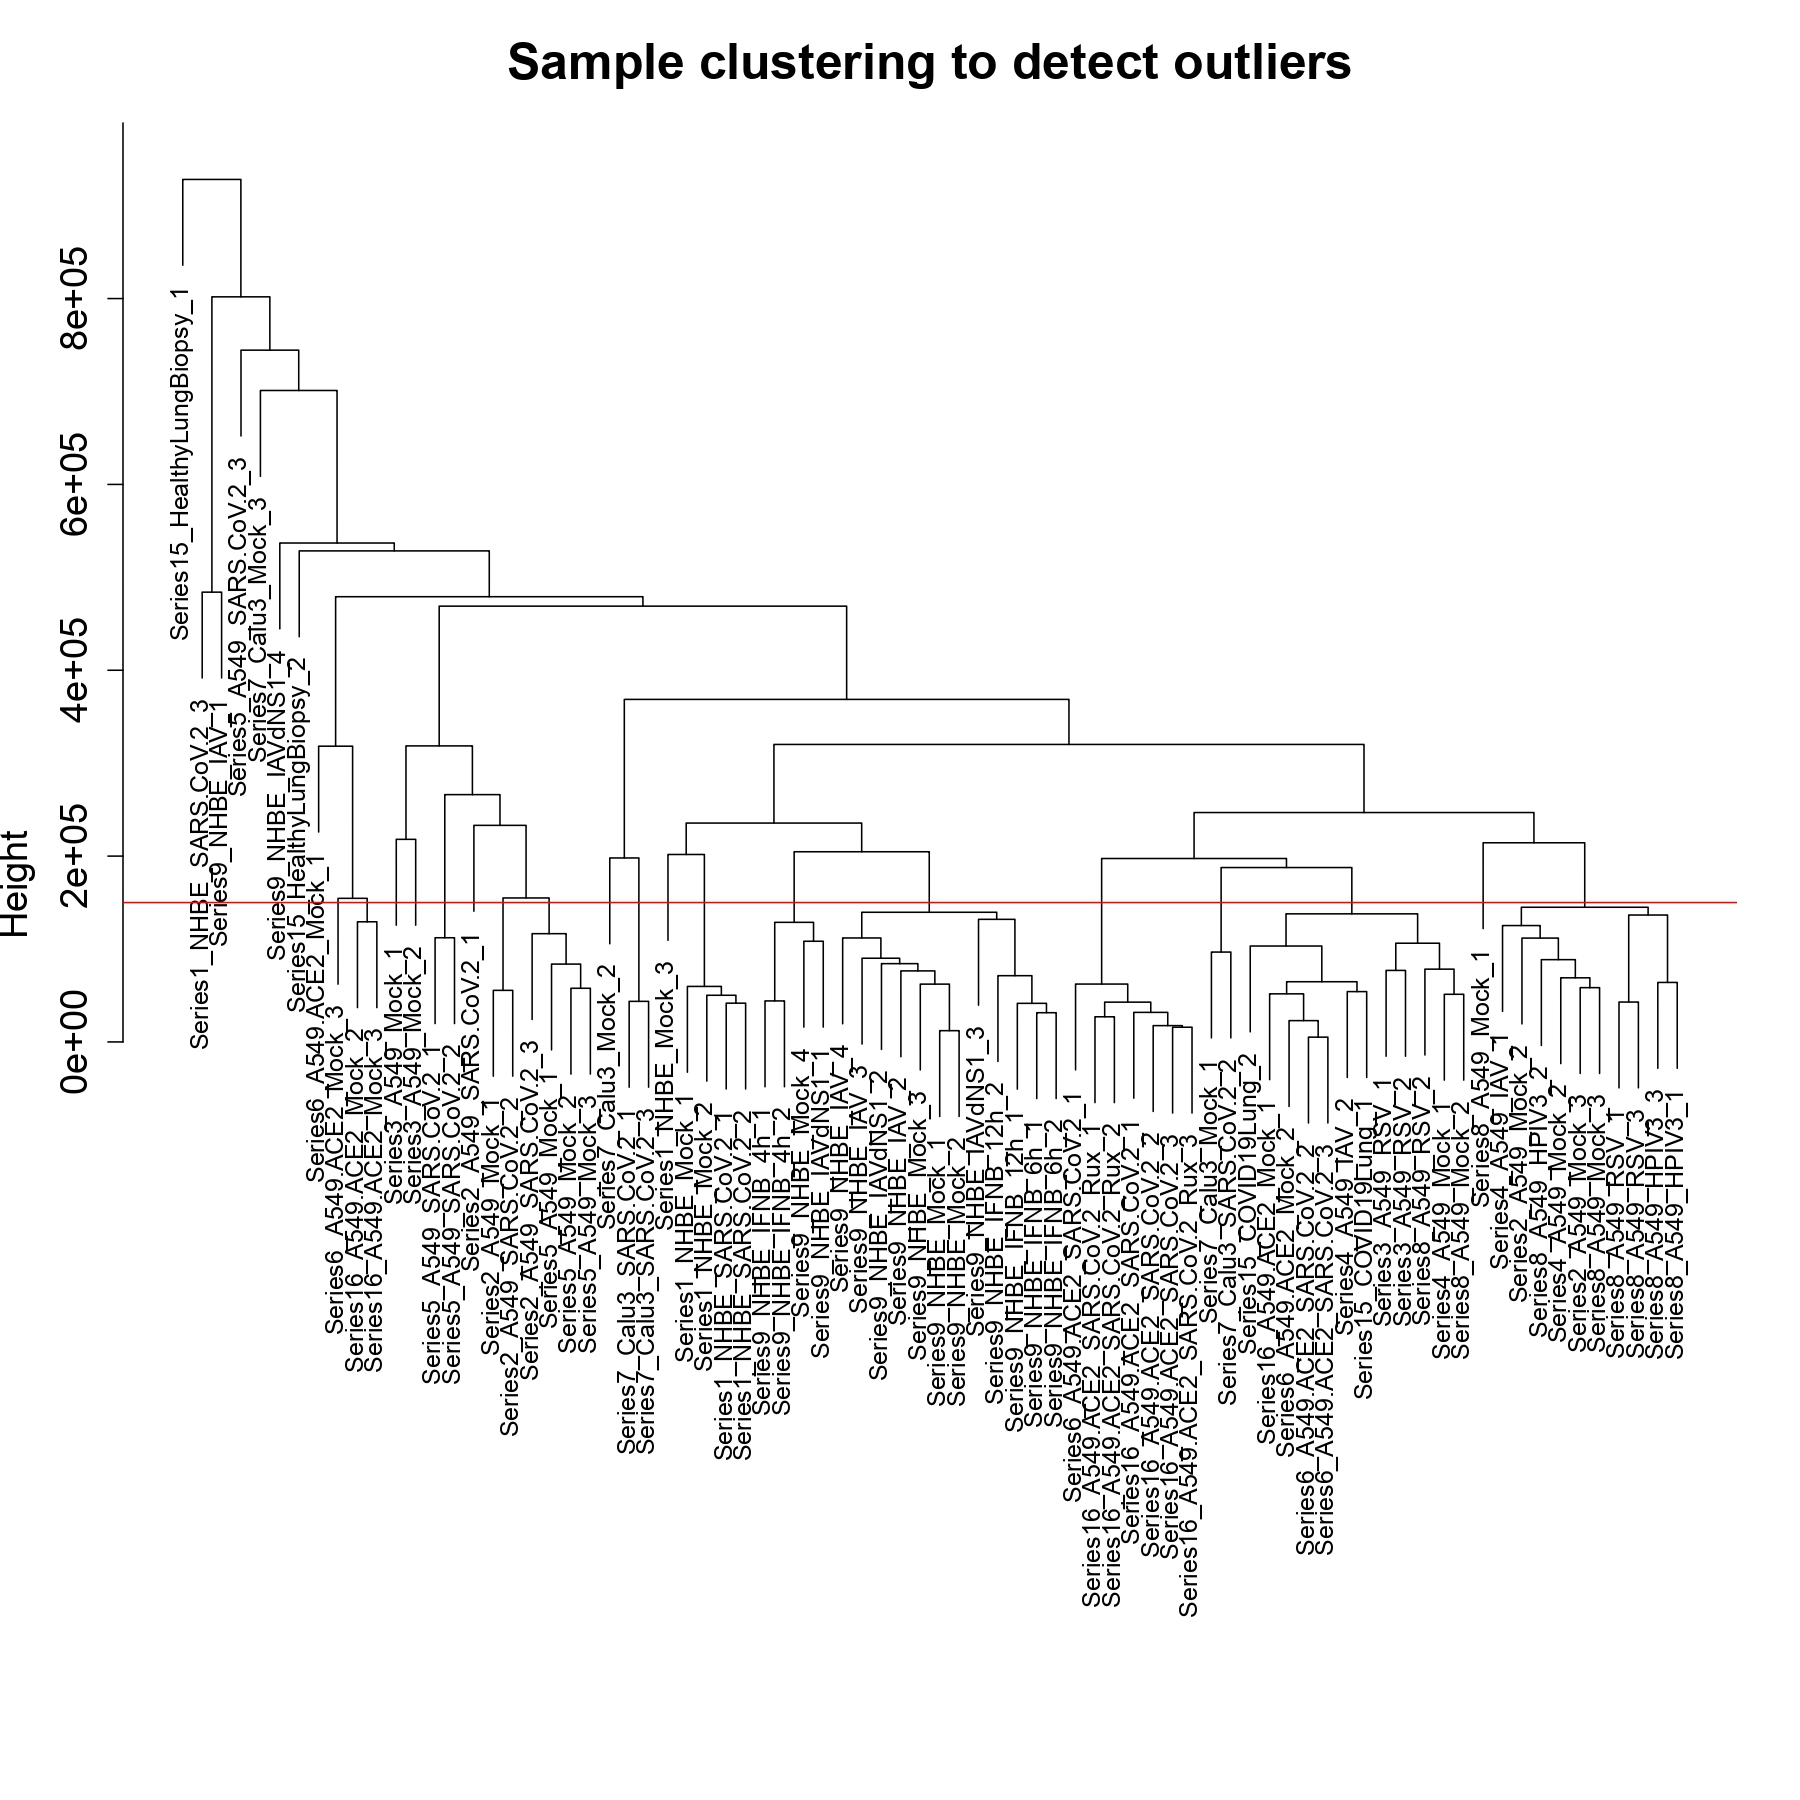
\includegraphics[width=0.9\textwidth]{figures/sampleClustering.jpg}}
	\caption{Sample Clustering}
	\label{fig:sample_clustering}
\end{figure}

Para el análisis de la topología de la red, lo primero que hemos hecho a nivel de implementación es la selección de umbrales. Posteriormente, transformamos el tipo de valores para todas las columnas, preocupándonos de que una función no detecta los valores si no son tipo \textit{NUMERIC}. Tras construir la red de genes y la identificaicón de los módulos, guardamos la información de la construcción de red.
	\section{Discusión}
Los datos presentados aquí sugieren que la respuesta al SARS-CoV-2 está desequilibrada con respecto al control de la replicación del virus frente a la activación de la respuesta inmunitaria adaptativa.

\begin{figure}[h]
	\fbox{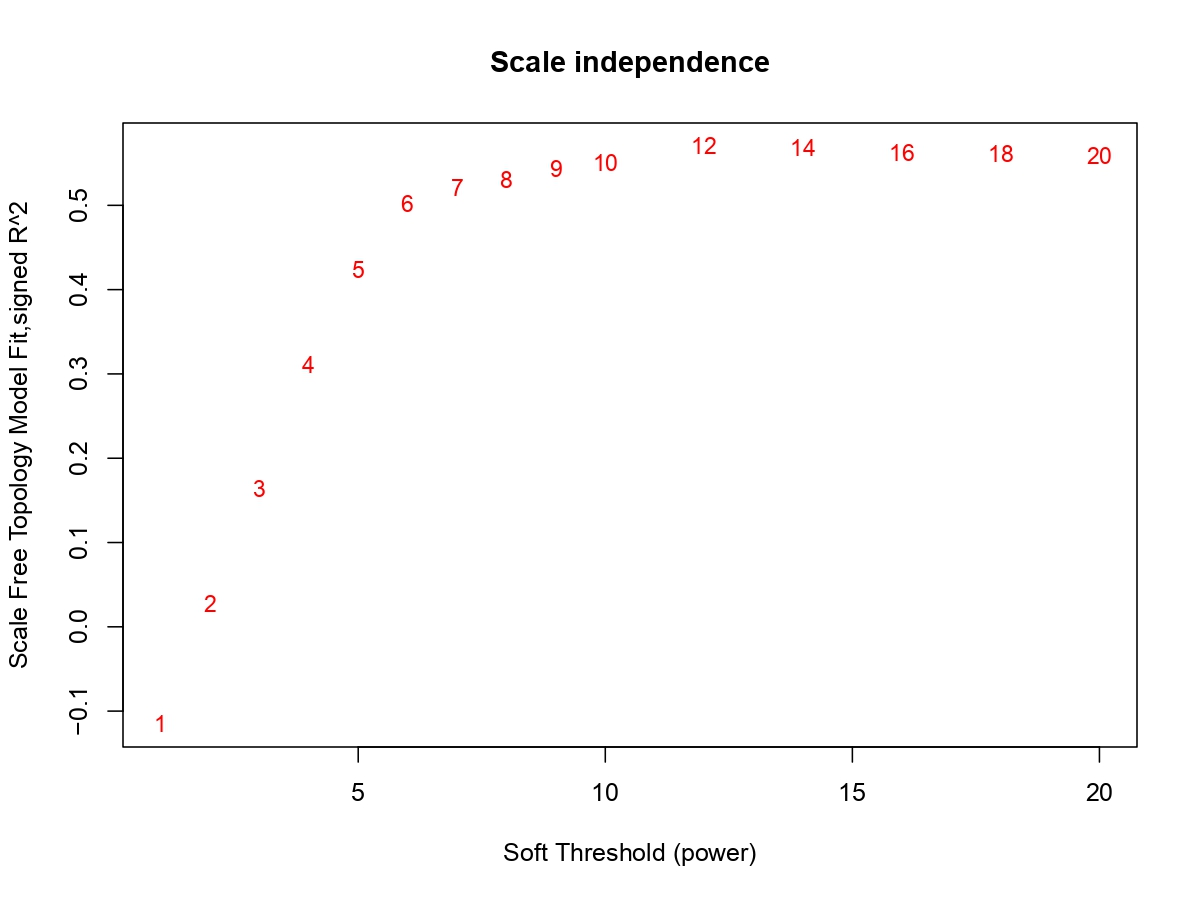
\includegraphics[width=0.9\textwidth]{figures/independenceScale_meanConnectivity1.jpg}}
	\caption{Independence Scale_mean Connectivity 1}
	\label{fig:sample_clustering}
\end{figure}

Dada esta dinámica, los tratamientos para la COVID-19 tienen menos que ver con la respuesta del IFN y más con el control de la inflamación. 

\begin{figure}[!]
	\fbox{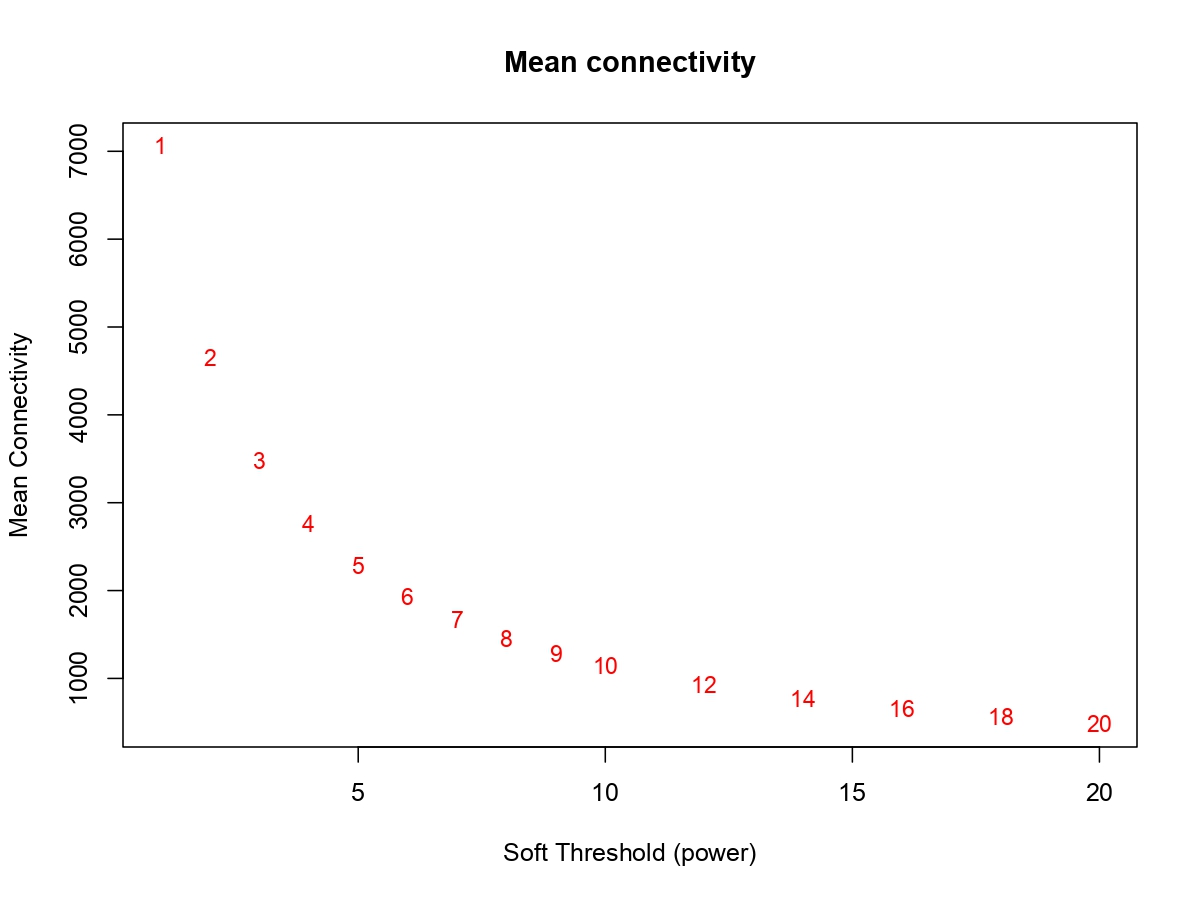
\includegraphics[width=0.9\textwidth]{figures/independenceScale_meanConnectivity2.jpg}}
	\caption{Independence Scale_mean Connectivity 2}
	\label{fig:sample_clustering}
\end{figure}



	\section{Conclusiones}




	
	
	%%%%%%%%%%%%%%%%%%%%%%%%%%%%%%%%%%%%%%%%%%%%%%
	%% OTRA INFORMACIÓN                         %%
	%%%%%%%%%%%%%%%%%%%%%%%%%%%%%%%%%%%%%%%%%%%%%%
	
	\begin{backmatter}
	
		\section*{Abreviaciones}%% if any
			\begin{itemize}
				\item NCBI: National Center for Biotechnology Information
				\item WGCNA: Weighted Correlation Network Analysis
			\end{itemize}
		
		\section*{Disponibilidad de datos y materiales}%% if any
			\href{https://github.com/smv762e/infectionResponse\_SARS-CoV2}{Proyecto en GitHub.}
					
		\section*{Contribución de los autores}
			C.L.A.C y J.A.H.C.: Encargados de la escritura de la memoria y resultados.
			\newline
			O.B. y S.M.V : Encargados de la escritura del código en R.

		
		%%%%%%%%%%%%%%%%%%%%%%%%%%%%%%%%%%%%%%%%%%%%%%%%%%%%%%%%%%%%%%%%%%%%%%%%%%%%%%%%%%%%%%%%
		%% BIBLIOGRAFIA: no teneis que tocar nada, solo sustituir el archivo bibliography.bib %%
		%% por el que hayais generado vosotros                                                %%
		%%%%%%%%%%%%%%%%%%%%%%%%%%%%%%%%%%%%%%%%%%%%%%%%%%%%%%%%%%%%%%%%%%%%%%%%%%%%%%%%%%%%%%%%
		
		\bibliographystyle{bmc-mathphys} % Style BST file (bmc-mathphys, vancouver, spbasic).
		\bibliography{bibliography}      % Bibliography file (usually '*.bib' )
	
	\end{backmatter}
\end{document}
